%%%%%%%%%%%%%%%%%%%%%%%%%%%%%%%%%%%%%%%%%
% Short Sectioned Assignment
% LaTeX Template
% Version 1.0 (5/5/12)
%
% This template has been downloaded from:
% http://www.LaTeXTemplates.com
%
% Original author:
% Frits Wenneker (http://www.howtotex.com)
%
% License:
% CC BY-NC-SA 3.0 (http://creativecommons.org/licenses/by-nc-sa/3.0/)
%
%%%%%%%%%%%%%%%%%%%%%%%%%%%%%%%%%%%%%%%%%

%----------------------------------------------------------------------------------------
%	PACKAGES AND OTHER DOCUMENT CONFIGURATIONS
%----------------------------------------------------------------------------------------

\documentclass[paper=a4, fontsize=11pt]{scrartcl} % A4 paper and 11pt font size

\usepackage[T1]{fontenc} % Use 8-bit encoding that has 256 glyphs
\usepackage{fourier} % Use the Adobe Utopia font for the document - comment this line to return to the LaTeX default
\usepackage[english]{babel} % English language/hyphenation
\usepackage{amsmath,amsfonts,amsthm} % Math packages

\usepackage{lipsum} % Used for inserting dummy 'Lorem ipsum' text into the template

\usepackage{sectsty} % Allows customizing section commands
\allsectionsfont{\centering \normalfont\scshape} % Make all sections centered, the default font and small caps

\usepackage{fancyhdr} % Custom headers and footers
\pagestyle{fancyplain} % Makes all pages in the document conform to the custom headers and footers
\fancyhead{} % No page header - if you want one, create it in the same way as the footers below
\fancyfoot[L]{} % Empty left footer
\fancyfoot[C]{} % Empty center footer
\fancyfoot[R]{\thepage} % Page numbering for right footer
\renewcommand{\headrulewidth}{0pt} % Remove header underlines
\renewcommand{\footrulewidth}{0pt} % Remove footer underlines
\setlength{\headheight}{13.6pt} % Customize the height of the header

\numberwithin{equation}{section} % Number equations within sections (i.e. 1.1, 1.2, 2.1, 2.2 instead of 1, 2, 3, 4)
\numberwithin{figure}{section} % Number figures within sections (i.e. 1.1, 1.2, 2.1, 2.2 instead of 1, 2, 3, 4)
\numberwithin{table}{section} % Number tables within sections (i.e. 1.1, 1.2, 2.1, 2.2 instead of 1, 2, 3, 4)

%\setlength\parindent{0pt} % Removes all indentation from paragraphs - comment this line for an assignment with lots of text

    \newenvironment{myindentpar}[1]%
     {\begin{list}{}%
             {\setlength{\leftmargin}{#1}
              \setlength{\rightmargin}{#1}
              }%
             \item[]%
     }
     {\end{list}}
\usepackage{graphicx}

 \usepackage{listings}
 
%----------------------------------------------------------------------------------------
%	TITLE SECTION
%----------------------------------------------------------------------------------------

\newcommand{\horrule}[1]{\rule{\linewidth}{#1}} % Create horizontal rule command with 1 argument of height

\title{	
\normalfont \normalsize 
\textsc{University of Pittsburgh\\
CS 1501: Algorithm Implementation} \\ [25pt] % Your university, school and/or department name(s)
\horrule{0.5pt} \\[0.4cm] % Thin top horizontal rule
\huge Dynamically Cutting Cloths\\ % The assignment title
\horrule{2pt} \\[0.5cm] % Thick bottom horizontal rule
}

\author{Zach Sadler} % Your name

\date{\normalsize\today} % Today's date or a custom date

\begin{document}

\maketitle % Print the title

%----------------------------------------------------------------------------------------
%	PROBLEM 1
%----------------------------------------------------------------------------------------

\section{Problem Description}

The \emph{Cloth Cutting Problem} is an optimization problem with real-world applications:
\begin{myindentpar}{1cm}
A textile company has a rectangular sheet of cloth with dimensions \emph{width} x \emph{height}. The company also has a set of patterns, $\mathbf{P}$, each $\mathbf{P}_i$ with its own width, height, and value ($m_i$, $n_i$, and \emph{$v_i$} respectively).\\
The company can only make full length cuts on a given piece of cloth- at increments $ 1 \le i \le k$, where $k$ is either the cloth's full width or full height- so that each cut creates two rectangular subcloths.\\
Which sequence of cuts should the company make to maximize the total value of patterns created?
\end{myindentpar}
%
Obviously, the problem is trivial if there are no patterns or the cloth is of non-positive area, so assume that the width and height are positive for the cloth and each pattern, and that each pattern has a positive value. One more important detail is that neither the cloths nor the patterns may be rotated. For example, if one of the patterns is of size 2 x 5, one may not make a pattern of size $5$ x $2$ and attempt to sell it for the same value (or indeed, any value at all).

%------------------------------------------------

\subsection{Example}
Let $\mathbf{P}$ be a set of patterns, as explained above. Let \emph{Subproblem}(subWidth, subHeight) be the maximum total value for a cloth of size subWidth x subHeight. Now we can give a concrete example.\\
\begin{figure}[ht!]
\centering
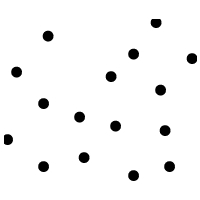
\includegraphics[width=40mm]{Figure_1.jpg}
\caption{The optimal cutting for the example problem given below}
\label{overflow}
\end{figure}
\\Let $\mathbf{P}_1$ be a 2 x 6 piece of cloth with value 4, let $\mathbf{P}_2$ be a 4 x 2 piece of cloth with value 3, and $\mathbf{P}_3$ be a 5 x 3 piece of cloth with value 5. If the initial cloth is of size 6 x 6, then the optimal value is created by a vertical cut at $x = 2$, and three horizontal cuts, at $y = 2$, $y = 4$, and $y = 6$, resulting in $v_1 + 3 \cdot v_3 = 13$ value (see Figure 1.1 for a visual solution).\\
\indent It is easy to see that this is a non-trivial problem, even for small amounts of patterns and a small total cloth size. For example, simply increasing the width by 1 and keeping the same set of patterns in the previous problem yields a much different result, as shown in Figure 1.2.
\begin{figure}[ht!]
\centering
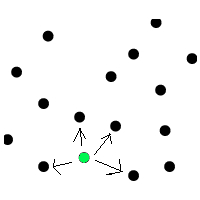
\includegraphics[width=50mm]{Figure_2.jpg}
\caption{A very different solution, despite very little change}
\label{overflow}
\end{figure}


%
%
%
\section{Naive Recursive Approach}
Clearly, if such a small change can alter the result even with just three patterns, it's apparent  that one will need to search exhaustively to find the solution. In the naive approach, one might think that knowing the previous problem will not impact the result of the current problem, as we saw in Figure 1.1 and 1.2. So, one would implement a top-down recursive approach as follows: \\

%%%%%%
\subsection{Code Listing - Naive}
\lstset{escapechar=\@}
\lstset{tabsize=2}
 \begin{lstlisting}
@\emph{Subproblem}@(subWidth, subHeight) {
	@\emph{patternMax, horizontalMax, verticalMax} $= 0$@ 
	for (@$i = 1 \dots$ \emph{numberOfPatterns}@)
		if (@\emph{patterns$_i$}@.value @$\ge$ \emph{patternMax}@)
			@\emph{patternsMax} $=$ \emph{patterns$_i$}@.value
			
	for (@$i = 1 \dots$ \emph{subWidth}@) {
		@\emph{temp} $=$ \emph{Subproblem}@(subWidth, i) + @\emph{Subproblem}@(subWidth, subHeight - i)
		if (@\emph{temp} $\ge$ \emph{horizontalMax}@) {	@\emph{horizontalMax} $=$ \emph{temp}@ }
	}
	for (@$i = 1 \dots$ \emph{subHeight}@) {
		@\emph{temp} $=$ \emph{Subproblem}@(i, subHeight) + @\emph{Subproblem}@(subWidth - i, subHeight)
		if (@\emph{temp} $\ge$ \emph{verticalMax}@) { @\emph{verticalMax} $=$ \emph{temp}@ }
	}
	return @\emph{max}@(patternMax, horizontalMax, verticalMax)
}
	
\end{lstlisting}   
%%%%%
\subsection{Analysis of Naive Recursive Algorithm}

The basic idea of the code listed above is to start with the current cloth, try each pattern on it and save the maximum value, then try each cut (recursively) both horizontally and vertically (saving the resulting maximum of each pair of subcloths), and return the maximum of these three values.\\
\indent This algorithm has major inefficiencies. Let's say that \emph{Subproblem}(m, n) took $\delta$ recursive calls to solve. Then to solve $\Delta$ = \emph{Subproblem}(m+1, n), we can see that along the way I will make a vertical cut at the first increment, leaving a cloth of size of m x n and another of size 1 x n. We already know that the cloth of size m x n will take $\delta$ recursive calls, and the cloth of size 1 x n will also require non-trivial work, and so naturally $\Delta > \delta$.\\
\indent However, we will also have to perform a vertical cut at increment m, yielding a cloth of size m x n and another of size 1 x n. So once again we will have to perform more than $\delta$ recursive calls, which means that $\Delta > 2 \cdot \delta$, or in other words, $T(n) = 2 \cdot T(n-1) + 2 \cdot \theta(n)$, (where $\theta(n)$ accounts for the calls required for a cloth of size 1 x n) which means this algorithm is exponential. \\
\indent Later in this paper we will see experimentation that confirms this analysis. Also, note that this analysis only took into account the adjustment of a single variable (either width or height- not both), increasing both values would result in an even worse case scenario, as \emph{Subproblem}(m+1, n+1) requires more than four times the recursive calls of \emph{Subproblem}(m, n).
%%%%%%%%

\section{Dynamic Bottom-up Approach}

Our naive algorithm has some serious issues stemming from the fact that it repeats so many of the same subproblems. Consider if, instead of starting from the largest problem and continuously breaking it down into the same sized subproblems again and again, we reversed our thought process. If we start from the smallest size and work our way up, we can keep track of the results of these smaller subproblems and then we can just look up the answer later instead of recalculating each time. Instead of solving the same subproblem (like 1x1) for every single larger subcloth, we would only have to solve it once and then remember the value, \\
\indent This type of approach would dramatically reduce the number of recursive calls needed, so surely it must require some dramatic changes in our code, right?
%%%%%

\subsection{Code Listing 2 - Dynamic}
In order to make our program dynamic, we must make the following changes:\\
\begin{lstlisting}
// stores the results of subproblem a x b in memos[a][b]
int [][] @\emph{memos} = new int[width + 1][height + 1]@

// starts from the bottom, storing memos as we find answers to subproblems
@\emph{Optimize}@() {
	// first initialize the memos to -1 as a flag to know we haven't been there yet
	for (@$i = 1 \dots$ \emph{width}@) 	
		for (@$j = 1 \dots$ \emph{height}@) 
			@\emph{memos}@[i][j] = -1
			
	// then start solving the subproblems and overwrite the flags with answers
	for (@$i = 1 \dots$ \emph{width}@) 	
		for (@$j = 1 \dots$ \emph{height}@) 
			@\emph{memos}@[i][j] = Subvalue(i, j)
}

@\emph{Subvalue}@(subWidth, subHeight) {
	if (@\emph{memos}@[subWidth][subHeight] > -1) {
		return @\emph{memos}@[subWidth][subHeight]
	}	
	@$\cdots$@
	// code from Subproblem before
	@$\cdots$@
}
\end{lstlisting}
%%%%%%%%


\subsection{Analysis of Dynamic Bottom-up Algorithm}

Wait, what? That's all the changes we make? It hardly seems like anything at all, so let's see if the runtime changed to any noticieable degree. \\ 
\indent As before, let's say that \emph{Subvalue}(m, n) took $\delta$ recursive calls. Then to solve $\Delta = $ \emph{Subvalue}(m + 1, n), we can see that we will take $\delta$ calls to solve up to a m x n subcloth. From there, if we make any vertical cut on the cloth of size (m + 1) x n then we will be at a previously solved subproblem, and finished after a constant-time lookup from the memos. Thus we just have to solve (from the bottom up), the cloths of size (m + 1) x \emph{i}, for $1 \le i \le n$, which will take $\theta$(n) because of memoization. So our recurrence relation is $T(n) = T(n-1) + c \cdot \theta(n)$, (for some constant $c$) which is quadratic. \\
\indent As another way of looking at it, just consider that we call Subvalue() $n \cdot m$ times, and while there is some additional recursion going on within those calls, with the memoization happening at constant-speed, the 'extra' recursion becomes negligible and the full algorithm takes $\Theta(n^2)$ time.  


%%%%%%%%%

\subsection{Technical Issues}
The code listing provided is almost exactly what I have in my submitted project (which received full credit), and so it really is as easy as it sounds. However, one might have noticed that this solution only gives the \emph{value} of the optimal cloth cutting sequence; not the sequence of cuts itself.\\
\indent In order to track the proper sequence of cuts, a little more bookkeeping is required. I have a class called 'Cut' which stores information about the best cuts which were found at each subproblem. 'Cut' tracks whether it was vertical or horizontal, the size of the cloth it cut, the position it cut (the increment from $1$ to the width or height), and the absolute offset of the subcloth compared to the original, full cloth. When I return the maximum value of \emph{patternMax}, \emph{horizontalMax}, and \emph{verticalMax}, if I made a horizontal or vertical cut I store the information about the current subproblem to an ArrayList of Cuts. Remember that since we only solve each subproblem once, this means that there will be a \emph{unique} cut for each $(x, y) \in width \times height$. \\
\indent Then, after I've solved all the subproblems and filled out my 2D array of memos, I do one final run from top to bottom. I retreive the cut corresponding to the largest suproblem, then using the information stored inside it I retrieve the next cut recursively (by adjusting my current subWidth and subHeight by where I made the cut) and keep track of my absolute offset from the origin, to be able to display it later graphically. As an example, if the cut on a subcloth of size 20 x 20 is a vertical cut with 'position' $= 3$ then I will recursively retrieve the cut for subcloth size 17 x 20 (which then has absolute offset $(3, 0)$), and after backtracing, recursively retrieve the cut for subcloth size 3 x 20 (which has absolute offset $(0, 0)$).   \\
\indent I recognize that this final run does cause some overhead, but it is very minimal compared to the \emph{Subvalue} method, which is itself very minimal compared to the naive approach.
%%%%%%%%%

\section{Results from Experimentation}
I adjusted my program so that I could turn memoization on and off, so that I could compare the number of recursive calls made when memoization was enabled versus disabled. The results were \textbf{truly staggering}, and confirmed my analyses of the runtimes:

\begin{table}[h]
\caption{Results from a Small Set of Experiments}
\centering
    \begin{tabular}{|l|l|l|l|l|l|l|}
        \hline
        Item    & 2 x 5 & 3 x 5 & 4 x 5 & 6 x 5  & 8 x 5    & 10 x 5    \\ \hline
        Memoized & 60    & 105   & 160   & 300    & 480      & 700       \\ 
        Naive    & 1,052  & 6,573  & 35,224 & 786,548 & 14,420,144 & 234,156,620 \\
        \hline									
    \end{tabular}
\end{table}

These results were calculated while running the program with the same dataset (four patterns: $\mathbf{P}_1$ a 2 x 2 with value 1; $\mathbf{P}_2$ a 2 x 6 with value 4; and $\mathbf{P}_3$ a 4 x2 with value 3; $\mathbf{P}_4$ a 5 x 3 with value 5). I ran each test three times to confirm the results, although there is no randomness to this deterministic algorithm, so there is no need for uncertainty about the number of recursive calls required.

These are the values (the maximum amount of money to be earned from the cloth) for each size: 
\begin{table}[h]
\caption{The Maximum Value to be Gained }
\centering
    \begin{tabular}{|l|l|l|l|l|l|l|}
        \hline
        Capacity & 2 x 5 & 3 x 5 & 4 x 5 & 6 x 5 & 8 x 5 & 10 x 5 \\ \hline
        Value    & 2     & 2     & 6     & 9     & 12    & 17     \\
        \hline
    \end{tabular}
\end{table}

\subsection{Memoized Experiment Analysis}
Using the data provided in Table 4.1, I found a quadratic formula that matches the data points for the memoized algorithm ($R$ and $R^2$ values of 1): 
\[
	5x^2 + 20x + 6.818 \cdot 10^{-14}
\]
\begin{figure}[ht!]
\centering
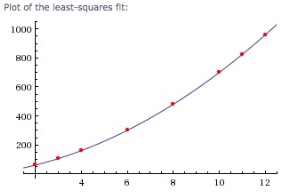
\includegraphics[width=100mm]{Figure_3.jpg}
\caption{The curve of $5x^2 + 20x + 6.818 \cdot 10^{-14}$ intersecting each data point}
\label{overflow}
\end{figure}\\
Although this is a relatively small data set it is evident that the memoized approach has a quadratic runtime.

\subsection{Naive Experiment Analysis}
Similarly, there is an exponential function that matches the data points for the naive algorithm (again, $R$ and $R^2$ values of 1):
\[
	206.505\mathbf{e}^{1.39412x}
\]
\begin{figure}[h]
\centering
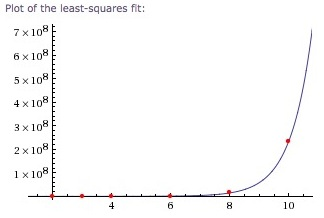
\includegraphics[width=100mm]{Figure_4.jpg}
\caption{The curve of $206.505\mathbf{e}^{1.39412x}$ intersecting each data point}
\label{overflow}
\end{figure} \\
This is an obviously exponential function, if the data points were not enough of a clue to begin with.

\section{A Quick Aside}
In case the graphs and the small experiment still did not give you a scale of the enormous numbers in play with the exponential function, consider the following:
\[
	206.505\mathbf{e}^{1.39412 \cdot \mathbf{20}} = 2.66 \cdot 10^{14}
\]
that means that if we simply double the width of the cloth used in the final experiment (from 10 x 5 to 20 x 5), we get a number so large that if it took a \textbf{millisecond} to do each recursive call, then it would still take about eight and a half thousand years to compute the answer. \\
\indent This is why it's important to find an efficient algorithm, because with the dynamic approach:
\[
	5 \cdot \mathbf{20}^2 + 20 \cdot \mathbf{20} + 6.818 \cdot 10^{-14} = 2400
\]
which means that if each recursive call took \textbf{3 years} the dynamic algorithm would \emph{still} beat the naive approach.\\
\indent The carpenter says to measure twice and cut once. The computer scientist says to make a program that can measure 2400 times in an instant, cut 8 times, and maximize your profit.






\end{document}